\documentclass[11pt]{article}

\usepackage[a4paper,margin=25mm,headheight=15pt]{geometry}
\usepackage[T1]{fontenc}
\usepackage{lmodern}
\usepackage{microtype}
\usepackage{xcolor}
\usepackage{graphicx}
\usepackage{booktabs}
\usepackage{longtable}
\usepackage{array}
\usepackage{enumitem}
\usepackage{fancyhdr}
\usepackage{titlesec}
\usepackage{tikz}
\usetikzlibrary{arrows.meta,positioning}
\usepackage[hidelinks]{hyperref}

\definecolor{navy}{HTML}{17324D}
\definecolor{teal}{HTML}{1D7A78}
\definecolor{lightblue}{HTML}{EAF3F6}
\definecolor{muted}{HTML}{526577}

\hypersetup{
  colorlinks=true,
  linkcolor=navy,
  urlcolor=teal,
  pdftitle={MCP Ambulance Handoff Gateway Using HL7 FHIR},
  pdfauthor={Omair Gibreel},
  pdfsubject={COSC726 Week 5 Project Proposal}
}

\setlength{\parindent}{0pt}
\setlength{\parskip}{6pt}
\setlist{itemsep=2pt,topsep=4pt,leftmargin=*}
\renewcommand{\arraystretch}{1.18}
\titleformat{\section}{\Large\bfseries\color{navy}}{\thesection}{0.65em}{}
\titleformat{\subsection}{\large\bfseries\color{teal}}{\thesubsection}{0.65em}{}
\titleformat{\subsubsection}{\normalsize\bfseries\color{navy}}{\thesubsubsection}{0.65em}{}

\pagestyle{fancy}
\fancyhf{}
\lhead{\small COSC726 Project Proposal}
\rhead{\small Omair Gibreel}
\cfoot{\small\thepage}
\renewcommand{\headrulewidth}{0.4pt}

\newcommand{\proposalTitle}{MCP Ambulance Handoff Gateway Using HL7 FHIR}
\newcommand{\term}[1]{\texttt{#1}}

\begin{document}

\begin{titlepage}
  \thispagestyle{empty}
  \vspace*{22mm}
  {\color{teal}\rule{\textwidth}{2.2pt}}\\[14mm]
  {\Huge\bfseries\color{navy}\proposalTitle\par}
  \vspace{8mm}
  {\Large Project Proposal\par}
  \vspace{18mm}

  \begin{tabular}{@{}>{\bfseries\color{navy}}p{35mm}p{105mm}@{}}
    Student & Omair Gibreel \\
    Course & COSC726 - Agentic Artificial Intelligence \\
    Week & Week 5 \\
    Project topic & Model Context Protocol, ambulance handoff, and HL7 FHIR \\
    Dataset & Synthea FHIR R4 patients, NEMSIS field definitions, and manually generated synthetic ambulance events \\
  \end{tabular}

  \vfill
  \colorbox{lightblue}{%
    \begin{minipage}{0.93\textwidth}
      \vspace{3mm}
      \textbf{Safety boundary.} This project uses synthetic data only. It does not diagnose a patient, recommend treatment, calculate a medication dose, select a destination hospital, or dispatch an ambulance. A clinician remains responsible for reviewing and confirming every handoff.
      \vspace{3mm}
    \end{minipage}}
  \vfill
  {\color{teal}\rule{\textwidth}{2.2pt}}
\end{titlepage}

\tableofcontents
\newpage

\section{Project Summary}

I plan to build a Model Context Protocol (MCP) server that helps transfer a synthetic ambulance patient record to a receiving emergency department in HL7 FHIR format. The dataset will combine Synthea FHIR R4 patients, NEMSIS Version 3 field definitions, and manually generated synthetic ambulance events. The project will focus on interoperability and safety by validating the record, detecting missing handoff information, building a structured draft, enforcing patient-level authorization, and recording an audit trail.

The system will not diagnose a patient, recommend treatment, calculate a drug dose, choose a destination hospital, or dispatch an ambulance. A clinician will remain responsible for checking and confirming the handoff. All cases will be synthetic, so no real protected health information will enter the repository, model context, logs, or demonstration.

\section{Problem Statement}

Ambulance and hospital systems may represent the same event differently. A prehospital record can contain demographics, times, vital signs, interventions, medications, and a clinical narrative, but the receiving system needs that information in a predictable structure. A custom integration can work for one application while being difficult to reuse, validate, or audit.

HL7 FHIR provides standardized healthcare resources and a JSON representation for exchanging clinical information. MCP gives an AI host a standard way to discover server-provided tools, resources, and prompt templates. This project combines them: FHIR standardizes the healthcare data, while MCP standardizes how an agent accesses validation and handoff capabilities.

The project is not intended to prove that an AI model can replace a paramedic or emergency clinician. It asks whether an MCP server can make a narrow ambulance handoff workflow more interoperable, complete, and auditable while keeping safety decisions outside the model.

\section{Dataset Strategy}

The project will use three complementary data sources rather than assuming that one dataset contains the complete ambulance-to-hospital journey.

\subsection{Synthea FHIR R4 Patients}

The starting point will be the official Synthea sample containing 100 synthetic patients in FHIR R4 format. A deterministic script will select 20 patients and copy only the resources needed by the project. Synthea provides realistic longitudinal structure without using real protected health information, and its sample data can be included in the public repository.

\subsection{NEMSIS Field Definitions}

The NEMSIS Version 3 data dictionary will define the shape and meaning of the prehospital source record. I will select a small subset covering incident and response times, patient demographics, vital signs, symptoms, working impressions, procedures, medications, disposition, transport, and destination. The exact NEMSIS dictionary release and selected element identifiers will be recorded in the mapping file.

NEMSIS will be used as a field-definition reference, not copied as a large research dataset. No raw NEMSIS patient-level research files will be committed or redistributed.

\subsection{Manually Generated Ambulance Events}

I will attach 40 synthetic ambulance events to the selected Synthea patients. Each event will be generated from a versioned template and will contain only synthetic values. Twenty-eight will represent normal complete or incomplete handoffs. Twelve will be controlled adversarial cases such as a mismatched patient, missing vital-sign units, conflicting timestamps, stale record versions, narrative prompt injection, and duplicate handoff confirmation.

Every event will have four linked artifacts:

\begin{enumerate}
  \item the selected Synthea patient resources;
  \item the NEMSIS-inspired synthetic source event;
  \item the expected FHIR R4 handoff Bundle; and
  \item labels for missing fields, permitted tools, expected validation findings, and the expected stop condition.
\end{enumerate}

This design makes the data small enough for GitHub and Google Colab while keeping the mapping and safety evaluation reproducible.

\section{Research Questions}

\begin{enumerate}
  \item Can two independent MCP clients discover and use the same ambulance handoff capabilities without client-specific tool definitions?
  \item Can a NEMSIS-inspired synthetic ambulance event linked to a Synthea patient be mapped into a valid HL7 FHIR R4 Bundle without losing source fields or inventing clinical facts?
  \item Can deterministic completeness checks identify missing handoff data more reliably than asking a language model to notice it?
  \item Can server-side authorization, patient matching, and clinician confirmation prevent wrong-patient disclosure and unapproved handoff submission?
  \item What latency and context-token overhead do MCP and FHIR validation add over direct custom JSON processing?
\end{enumerate}

\section{Proposed Workflow and Architecture}

\begin{enumerate}
  \item A Synthea FHIR R4 patient and its linked synthetic ambulance event are loaded from the versioned evaluation dataset.
  \item A deterministic mapper applies the documented NEMSIS-to-FHIR field map and creates a FHIR R4 document Bundle.
  \item The MCP server exposes the authorized case as a resource.
  \item The client calls validation and completeness tools before requesting a handoff draft.
  \item A language model may summarize the already grounded fields into a MIST- or SBAR-style draft, with source references attached.
  \item A simulated clinician confirmation is required before the handoff can be marked as sent.
  \item The server records validation results, confirmation, receiving facility, timestamps, and provenance in a redacted audit trail.
\end{enumerate}

\begin{figure}[htbp]
\centering
\resizebox{\textwidth}{!}{%
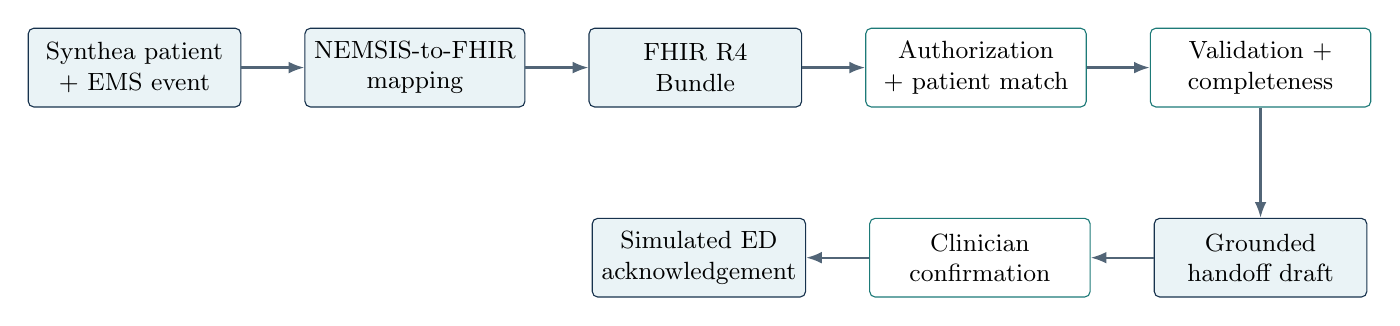
\begin{tikzpicture}[
  node distance=8mm,
  box/.style={draw=navy,rounded corners=2pt,fill=lightblue,align=center,minimum height=10mm,minimum width=27mm,font=\small},
  gate/.style={draw=teal,rounded corners=2pt,fill=white,align=center,minimum height=10mm,minimum width=28mm,font=\small},
  flow/.style={-{Latex[length=2mm]},thick,color=muted}
]
  \node[box] (source) {Synthea patient\\+ EMS event};
  \node[box,right=of source] (map) {NEMSIS-to-FHIR\\mapping};
  \node[box,right=of map] (bundle) {FHIR R4\\Bundle};
  \node[gate,right=of bundle] (auth) {Authorization\\+ patient match};
  \node[gate,right=of auth] (validate) {Validation +\\completeness};
  \node[box,below=14mm of validate] (draft) {Grounded\\handoff draft};
  \node[gate,left=of draft] (confirm) {Clinician\\confirmation};
  \node[box,left=of confirm] (ack) {Simulated ED\\acknowledgement};
  \draw[flow] (source) -- (map);
  \draw[flow] (map) -- (bundle);
  \draw[flow] (bundle) -- (auth);
  \draw[flow] (auth) -- (validate);
  \draw[flow] (validate) -- (draft);
  \draw[flow] (draft) -- (confirm);
  \draw[flow] (confirm) -- (ack);
\end{tikzpicture}}
\caption{Proposed ambulance handoff workflow. Deterministic controls protect every consequential step.}
\label{fig:workflow}
\end{figure}

\section{FHIR Data Model}

The implementation will target the published HL7 FHIR R4 specification and use a deliberately small profile suitable for the course project.

\begin{longtable}{@{}>{\raggedright\arraybackslash}p{38mm}>{\raggedright\arraybackslash}p{115mm}@{}}
\toprule
\textbf{FHIR resource} & \textbf{Use in the project} \\
\midrule
\endfirsthead
\toprule
\textbf{FHIR resource} & \textbf{Use in the project} \\
\midrule
\endhead
\term{Patient} & Synthetic identifier and limited demographics needed for matching. \\
\term{Encounter} & Ambulance incident and transfer-of-care context. \\
\term{Observation} & Timestamped vital signs with explicit values and units. \\
\term{ClinicalImpression} & Paramedic working impression, clearly marked as provisional. \\
\term{MedicationAdministration} & Medication already administered, not a recommendation. \\
\term{Procedure} & Intervention already performed. \\
\term{Practitioner}, \term{Organization} & Synthetic ambulance crew and receiving organization. \\
\term{Location} & Incident and receiving locations using synthetic identifiers. \\
\term{Composition}, \term{Bundle} & Structured handoff document and contained resources. \\
\term{Provenance}, \term{AuditEvent} & Source, transformation, access, and confirmation records. \\
\bottomrule
\end{longtable}

Every generated value will either point to a source field or be a documented transformation. Missing source data will remain absent or use the appropriate FHIR representation; the model will not fill gaps by guessing.

\section{MCP Capabilities}

\subsection{Tools}

\begin{longtable}{@{}>{\raggedright\arraybackslash}p{44mm}>{\raggedright\arraybackslash}p{22mm}>{\raggedright\arraybackslash}p{87mm}@{}}
\toprule
\textbf{Tool} & \textbf{Tier} & \textbf{Behaviour} \\
\midrule
\endfirsthead
\toprule
\textbf{Tool} & \textbf{Tier} & \textbf{Behaviour} \\
\midrule
\endhead
\path{validate_fhir_bundle} & Read & Runs structural and project-profile validation and returns exact issues. \\
\path{get_ambulance_case} & Read & Returns the authorized synthetic case and its source version. \\
\path{check_handoff_completeness} & Read & Reports missing identity, timing, vital, intervention, and provenance fields. \\
\path{create_handoff_draft} & Read & Creates a grounded MIST- or SBAR-style draft with evidence references. \\
\path{confirm_handoff} & Consequential & Marks a simulated handoff as sent only with clinician confirmation and an idempotency key. \\
\path{record_ed_acknowledgement} & Write & Records a simulated receiving-department acknowledgement. \\
\bottomrule
\end{longtable}

There will be no tool for diagnosis, treatment selection, medication ordering, dose calculation, destination selection, or ambulance dispatch.

\subsection{Resources}

\begin{itemize}
  \item \path{ambulance://cases/{case_id}/source} - authorized synthetic source record;
  \item \path{ambulance://cases/{case_id}/fhir} - mapped FHIR Bundle;
  \item \path{ambulance://cases/{case_id}/validation} - current validation report;
  \item \path{ambulance://cases/{case_id}/audit} - redacted audit trail; and
  \item \path{ambulance://profiles/handoff-r4} - project data dictionary and profile rules.
\end{itemize}

\subsection{Prompts}

\begin{itemize}
  \item \path{prepare_mist_handoff} - drafts a concise handoff from validated evidence;
  \item \path{prepare_sbar_handoff} - provides an alternate structured handoff format; and
  \item \path{explain_validation_failure} - explains missing or invalid fields without inventing replacements.
\end{itemize}

The prompt templates are guidance, not security controls. The server will apply the same validation and authorization even if a client ignores them.

\section{Safety, Security, and Privacy}

\begin{itemize}
  \item The dataset will contain synthetic patients only. No real names, addresses, record numbers, narratives, or images will be used.
  \item The authenticated server will create the patient and user scope. The model cannot gain access by passing a patient identifier or claiming a clinical role in a tool argument.
  \item Every read will check that the case belongs to the authorized synthetic tenant and current handoff session.
  \item Patient matching will use more than a free-text name. The evaluation will include similar identifiers and deliberately mismatched cases.
  \item Clinical narrative, FHIR text fields, and tool results will be treated as untrusted data because they can contain prompt injection.
  \item Vital values will retain timestamps and explicit units. The system will not silently convert or merge conflicting observations.
  \item A draft cannot be confirmed while required identifiers, provenance, or validation gates are missing.
  \item \path{confirm_handoff} will require a clinician-confirmation claim, receiving organization, current case version, and idempotency key. It will not accept a confirmation requested only by the model.
  \item Logs will use case and run identifiers and will avoid raw patient text. Secrets and authorization tokens will never be committed.
  \item Local development will use \term{stdio}. Streamable HTTP tests will validate origins, bind locally, and use scoped test authorization.
\end{itemize}

\section{Evaluation Dataset}

I will create 40 synthetic ambulance cases linked to 20 deterministically selected patients from the Synthea 100-patient FHIR R4 sample:

\begin{itemize}
  \item 28 normal cases covering complete and incomplete handoffs, repeated vital signs, administered medications, procedures, and receiving acknowledgements; and
  \item 12 adversarial cases covering wrong-patient identifiers, missing units, impossible timestamps, stale case versions, duplicate confirmation, hidden instructions in narrative text, cross-patient access, and requests to invent missing clinical facts.
\end{itemize}

Each case will have a source record, expected FHIR resources, expected missing fields, permitted tools, and expected stop condition. It will also record the source Synthea patient identifier, event-template version, selected NEMSIS field identifiers, mapping version, and FHIR profile version. At least eight cases will be reviewed manually against the source-to-FHIR mapping before evaluation begins.

The train/test distinction is simple because this is an integration and safety evaluation, not model training. Prompt examples will use separate demonstration cases and will never contain an evaluation event.

\section{Experimental Comparison}

The same cases will be run through four configurations:

\begin{enumerate}
  \item custom ambulance JSON processed by direct Python functions;
  \item FHIR mapping and validation without MCP;
  \item MCP plus FHIR schemas without patient and confirmation gates; and
  \item secured MCP plus FHIR with all authorization, provenance, and confirmation gates enabled.
\end{enumerate}

The comparison will report:

\begin{itemize}
  \item FHIR structural and project-profile validity;
  \item source-to-FHIR field mapping accuracy;
  \item missing-field detection precision and recall;
  \item unsupported or invented clinical fields, with a target of zero;
  \item wrong-patient or cross-tenant disclosures, with a target of zero;
  \item unconfirmed handoffs marked sent, with a target of zero;
  \item duplicate handoffs after retry, with a target of zero;
  \item correct completion and safe-block rates;
  \item p50 and p95 local latency;
  \item context tokens per case; and
  \item capability discovery and execution from at least two MCP clients.
\end{itemize}

The model name, MCP SDK version, FHIR version, profile version, prompt version, transport, and case-set commit will be recorded beside every result.

\section{Google Colab and Reproducibility}

The project will include a Google Colab notebook that installs pinned Python dependencies, downloads or reads the pinned Synthea FHIR R4 sample, verifies its checksum, generates the ambulance events from versioned templates, starts the MCP server locally, runs the client, validates the FHIR Bundles, displays the evaluation table, and shuts the server down cleanly. A deterministic fake model client will run every safety test without an API key. An optional open-weight model section may be used only for handoff wording, not for validation or authorization.

No notebook cell will depend on a path from my own computer. A fresh Colab runtime should be able to reproduce the deterministic results from the cloned repository.

\section{Planned Repository Structure}

\begin{verbatim}
week05/
|-- project_proposal.md
|-- project_proposal.tex
|-- output/pdf/project_proposal.pdf
`-- proposal_checklist.md
project/
|-- README.md
|-- requirements.txt
|-- ambulance_mcp/
|   |-- server.py
|   |-- domain.py
|   |-- fhir_mapping.py
|   |-- validation.py
|   |-- authorization.py
|   `-- audit.py
|-- data/
|   |-- source/synthea_patients/
|   |-- source/ambulance_events/
|   |-- expected/fhir_bundles/
|   `-- labels/evaluation_labels.json
|-- mappings/nemsis_to_fhir.csv
|-- scripts/build_dataset.py
|-- profiles/handoff-r4.json
|-- tests/
`-- notebooks/ambulance_mcp_colab.ipynb
\end{verbatim}

\section{Schedule}

\begin{longtable}{@{}>{\bfseries}p{18mm}p{137mm}@{}}
\toprule
\textbf{Week} & \textbf{Planned result} \\
\midrule
5 & Proposal, scope, safety boundaries, and research questions. \\
6 & Pin Synthea sample, select patients, define NEMSIS fields, and write the threat model. \\
7 & Build the FHIR mapper, validator, and deterministic tests. \\
8 & Build the MCP \term{stdio} server with tools, resources, and prompts. \\
9 & Add patient-scoped authorization, confirmation gate, and audit events. \\
10 & Run Streamable HTTP and adversarial testing. \\
11 & Produce baselines, measurements, error analysis, and the Colab notebook. \\
12 & Complete the final report, reproducible release, and demonstration. \\
\bottomrule
\end{longtable}

\section{Deliverables}

\begin{itemize}
  \item Python MCP server implementing the ambulance handoff capabilities;
  \item selected Synthea FHIR R4 patient subset;
  \item manually generated NEMSIS-inspired ambulance events and expected FHIR Bundles;
  \item versioned NEMSIS-to-FHIR mapping table and dataset-generation script;
  \item FHIR mapping and validation rules;
  \item two MCP clients, or one client plus the MCP Inspector;
  \item Google Colab demonstration notebook;
  \item automated normal, authorization, and adversarial tests;
  \item threat model and privacy design;
  \item accuracy, safety, latency, and token comparison table; and
  \item final report and demonstration.
\end{itemize}

\section{Risks and Fallback Plan}

FHIR can become too broad for one course project. I will restrict the profile to the listed resources and fields rather than attempting a complete electronic patient care record. If a full terminology server is unavailable, the project will validate a documented local value set and report that limitation. If Streamable HTTP takes too much time, the tested core will remain \term{stdio} and the HTTP demonstration will stay local. If a real model is slow or unreliable, the deterministic client will still demonstrate all protocol, validation, authorization, and audit requirements.

The NEMSIS standard will be used as a reference for prehospital field names, but full NEMSIS certification and a complete NEMSIS-to-FHIR implementation are out of scope. The project will publish a small, explicit mapping table instead. If the Synthea download changes, the build script will fail its checksum check instead of silently creating a different dataset.

\section{Success Criteria}

The project will be considered successful when a fresh Colab runtime can run the documented demonstration; two clients can discover the same MCP capabilities; every generated handoff Bundle passes the declared FHIR profile; normal cases preserve their expected source fields; missing fields are reported without invention; cross-patient reads and unconfirmed submissions always fail; repeated confirmation does not create duplicates; and the final report measures what MCP and FHIR added instead of only showing that the server starts.

\newpage
\section{References}

\begin{enumerate}[label={[\arabic*]}]
  \item MITRE, ``Synthea Synthetic Patient Downloads.'' \url{https://synthea.mitre.org/downloads}
  \item HL7 International, ``FHIR Release 4 Specification.'' \url{https://hl7.org/fhir/R4/}
  \item HL7 International, ``Patient Resource.'' \url{https://hl7.org/fhir/R4/patient.html}
  \item HL7 International, ``Observation Resource.'' \url{https://hl7.org/fhir/R4/observation.html}
  \item HL7 International, ``Encounter Resource.'' \url{https://hl7.org/fhir/R4/encounter.html}
  \item HL7 International, ``Bundle Resource.'' \url{https://hl7.org/fhir/R4/bundle.html}
  \item HL7 International, ``Provenance Resource.'' \url{https://hl7.org/fhir/R4/provenance.html}
  \item HL7 International, ``AuditEvent Resource.'' \url{https://hl7.org/fhir/R4/auditevent.html}
  \item HL7 International, ``SMART App Launch Implementation Guide.'' \url{https://hl7.org/fhir/smart-app-launch/}
  \item NEMSIS, ``Version 3 Technical Resources.'' \url{https://nemsis.org/technical-resources/version-3/}
  \item NEMSIS, ``Version 3 Data Dictionaries.'' \url{https://nemsis.org/technical-resources/version-3/version-3-data-dictionaries/}
  \item Model Context Protocol, ``Protocol Specification.'' \url{https://modelcontextprotocol.io/specification/latest}
  \item Model Context Protocol, ``Official Python SDK.'' \url{https://github.com/modelcontextprotocol/python-sdk}
  \item Model Context Protocol, ``Security Best Practices.'' \url{https://modelcontextprotocol.io/specification/latest/basic/security_best_practices}
\end{enumerate}

\end{document}
